\documentclass{beamer}

\usepackage{graphicx}
\usepackage{caption}
\usepackage{algorithm,algorithmic}

\mode<presentation>
{
  \usetheme{Darmstadt}

  \setbeamercovered{transparent}
}

\DeclareMathOperator*{\argmax}{arg\,max}
\DeclareMathOperator*{\argmin}{arg\,min}

\title{Gradient Coding}

\author{Runtian Zhu \\ \texttt{zhurt23@m.fudan.edu.cn}}

\date{2023.11.9}

\begin{document}

\captionsetup[figure]{labelformat=empty}

\begin{frame}
  \titlepage
\end{frame}

\section{Reference}

\begin{frame}{Reference}

\begin{itemize}
    \item R. Tandon, Q. Lei, A. G. Dimakis, and N. Karampatziakis, “\textbf{Gradient coding: Avoiding stragglers in distributed learning},” in International Conference on Machine Learning, PMLR, 2017, pp. 3368–3376.
\end{itemize}

\begin{figure}
    \centering
    \begin{minipage}[t]{.2\paperwidth}
        \centering
        
\includegraphics[width=\textwidth]{res/Rashish Tandon.jpg}
        \caption{Rashish Tandon}
    \end{minipage}
    \begin{minipage}[t]{.2\paperwidth}
        \centering
        
\includegraphics[width=\textwidth]{res/Qi Lei.jpg}
        \caption{Qi Lei}
    \end{minipage}
    \begin{minipage}[t]{.2\paperwidth}
        \centering
        
\includegraphics[width=\textwidth]{res/alexdimakis_sm.jpg}
        \caption{Alexandros G. Dimakis}
    \end{minipage}
    \begin{minipage}[t]{.2\paperwidth}
        \centering
        
\includegraphics[width=\textwidth]{res/Nikos Karampatziakis.jpg}
        \caption{Nikos Karampatziakis}
    \end{minipage}
\end{figure}

\end{frame}

\section{Background}

\begin{frame}
    \frametitle{Machine Learning: Regression}

    \begin{block}{Regression}
        Given a data set $D = \{(\boldsymbol{x}_1, \boldsymbol{y}_1), \dots, (\boldsymbol{x}_N, \boldsymbol{y}_N)\}$. The goal is to find a function $f$ from some function space $F$ such that
        $f$ fits $D$ best ($f(\boldsymbol{x}_i)\approx \boldsymbol{y}_i$).
    \end{block}

    \begin{example}
        \[D = \{(0, 0), (1, 1), (-1, 0)\}\] \\
        \[F = \{x^2 + ax + b \vert a, b \in \mathbb{R}\}\] \\
        \[f(x) = ?\]
    \end{example}

\end{frame}

\begin{frame}
    \frametitle{Machine Learning: Regression}

    \begin{block}{Regression}
        Given a data set $D = \{(\boldsymbol{x}_1, \boldsymbol{y}_1), \dots, (\boldsymbol{x}_N, \boldsymbol{y}_N)\}$. The goal is to find a function $f_{\hat{\boldsymbol{\theta}}}$ from some function space $F = \{f_{\boldsymbol{\theta}} \vert \boldsymbol{\theta} \in \mathbb{R}^m\}$ such that
        \[\hat{\boldsymbol{\theta}} = \argmin_{\boldsymbol{\theta}} L(\boldsymbol{\theta})\]
    \end{block}
    
    \begin{block}{Loss Function: Mean Squared Error (MSE)}
        \[L(\boldsymbol{\theta}) = \frac{1}{N}\sum_{i = 1}^{N} \lVert\boldsymbol{y}_i - f_{\boldsymbol{\theta}}(\boldsymbol{x}_i)\rVert^2\]
    \end{block}

    \[D = \{(0, 0), (1, 1), (-1, 0)\},\; F = \{x^2 + ax + b \vert a, b \in \mathbb{R}\}, \;\boldsymbol{\theta} = \begin{bmatrix}
        a \\
        b
    \end{bmatrix}\]

\end{frame}

\begin{frame}{Gradient Descent in Machine Learning}

\begin{example}
    \begin{figure}
        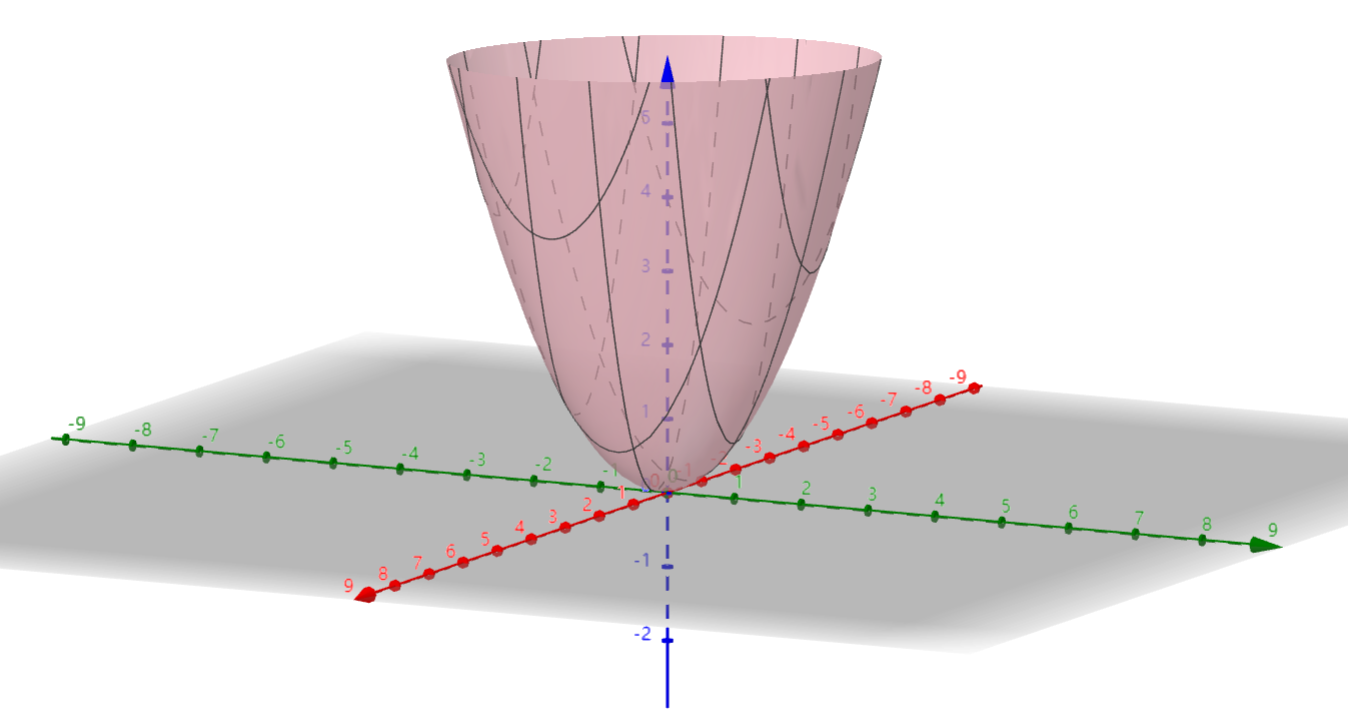
\includegraphics[height=.35\paperheight]{res/func3d.png}
    \end{figure}
    \[f(x, y) = \frac{1}{3}(1 - 2x + 3x^2 + 2y + 2y^2)\]
\end{example}

\begin{block}{Gradient Descent}
    \[\boldsymbol{\theta}_{k + 1} = \boldsymbol{\theta}_{k} - \alpha\boldsymbol{\nabla} L(\boldsymbol{\theta}_{k})\]
\end{block}

\end{frame}

\begin{frame}
    \frametitle{Linearity of Loss Functions and Gradients}


    \begin{block}{Gradient Descent}
        \[\boldsymbol{\theta}_{k + 1} = \boldsymbol{\theta}_{k} - \alpha\boldsymbol{\nabla} L(\boldsymbol{\theta}_{k})\]
    \end{block}
    
    \begin{block}{Loss Function: Mean Squared Error (MSE)}
        \[L(\boldsymbol{\theta}) = \frac{1}{N}\sum_{i = 1}^{N} \lVert\boldsymbol{y}_i - f_{\boldsymbol{\theta}}(\boldsymbol{x}_i)\rVert^2\]
        \[\boldsymbol{\nabla}L(\boldsymbol{\theta}) = \sum_{i = 1}^{N}\frac{1}{N}\frac{\partial\lVert\boldsymbol{y}_i - f_{\boldsymbol{\theta}}(\boldsymbol{x}_i)\rVert^2}{\partial\boldsymbol{\theta}}\]
    \end{block}

\end{frame}

\begin{frame}{Distributed Learning}{Straggler Problem}
    \begin{columns}
        \begin{column}{0.6\textwidth}
            \begin{block}{Problem Setting}
                Given data sets $D_1, \dots, D_k$ ($D_i$ can be viewed as a vector). Each round, a parameter $\boldsymbol{\theta}$ is given. Calculate $\boldsymbol{g}_{\boldsymbol{\theta}}(D_1) + \dots + \boldsymbol{g}_{\boldsymbol{\theta}}(D_k)$.
            \end{block}
            Problem:
            \begin{itemize}
                \item Some workers may be stragglers (work 5x slower)
            \end{itemize}
            
        \end{column}
        \begin{column}{0.48\textwidth}
            \begin{figure}
                \centering
                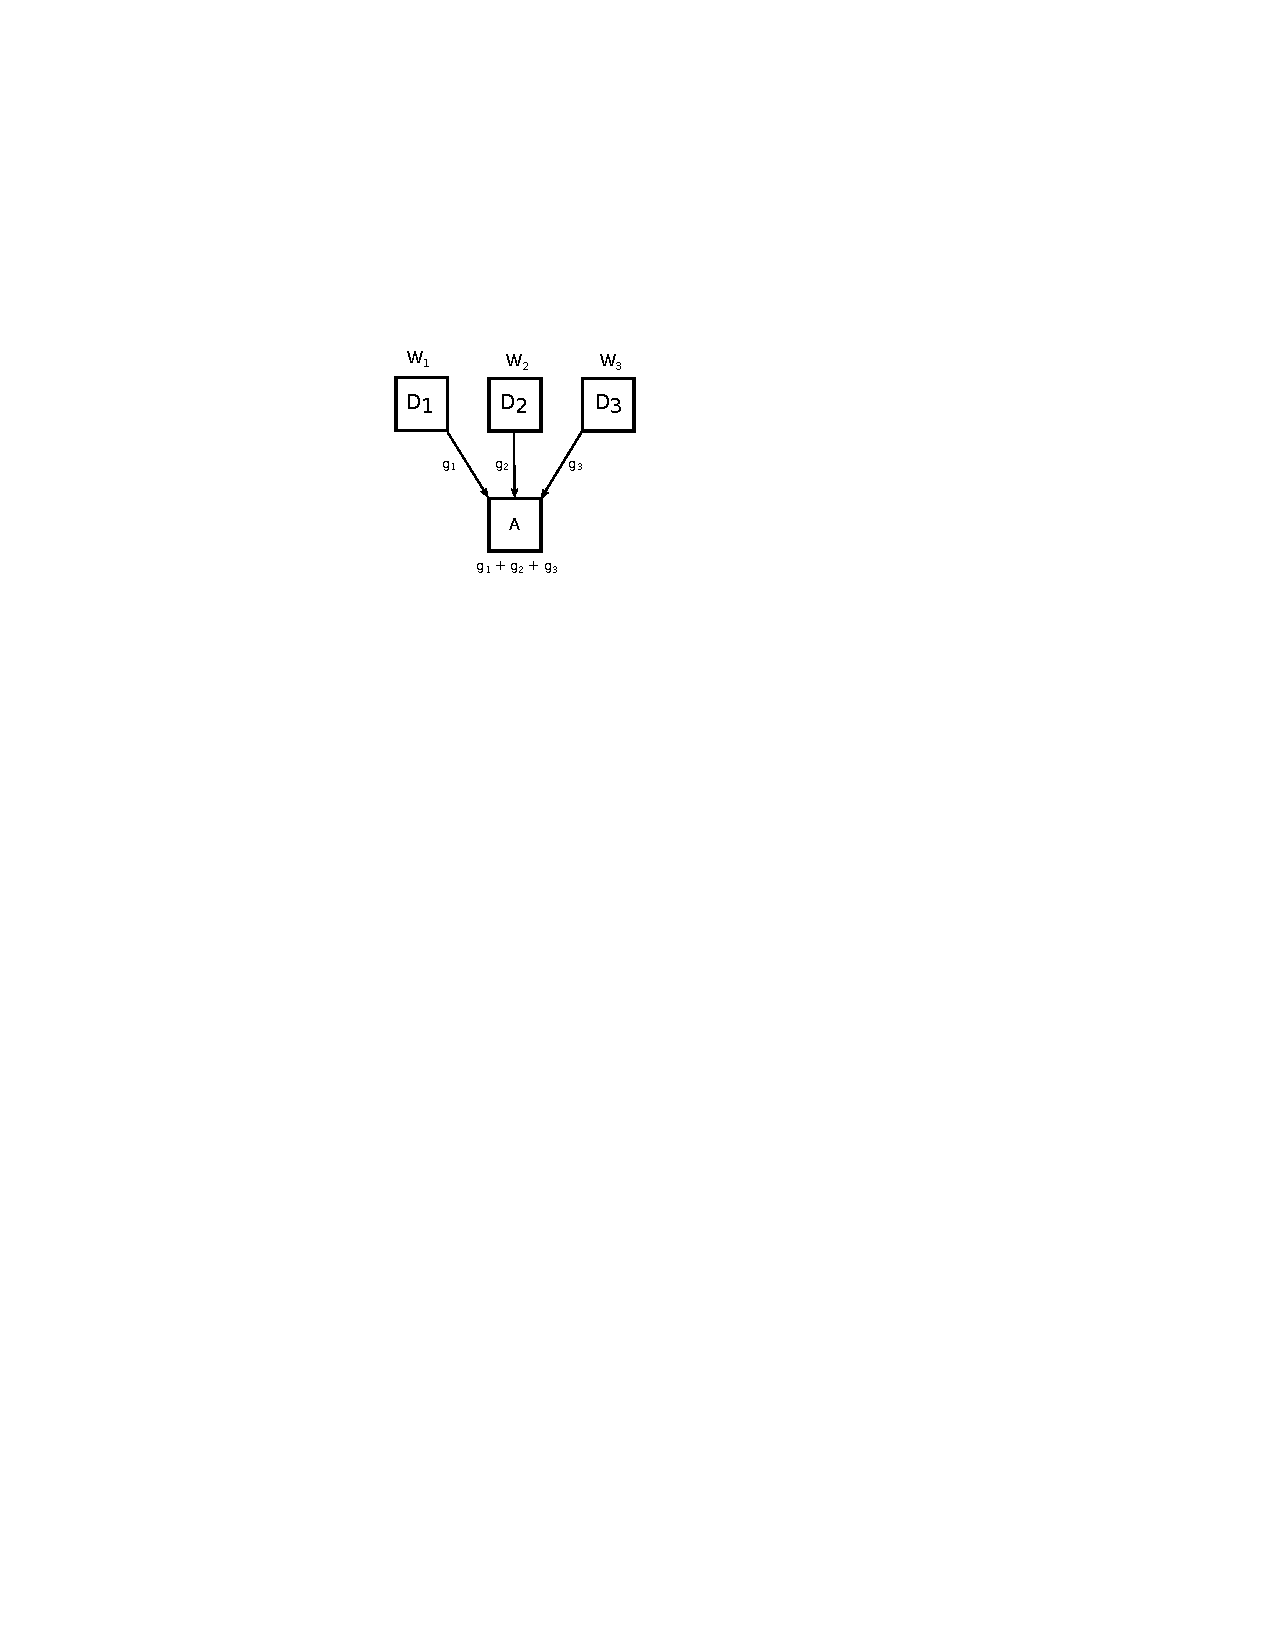
\includegraphics[height=.5\textheight]{res/distributed_learning.pdf}
            \end{figure}
        \end{column}
    \end{columns}
\end{frame}

\begin{frame}{Distributed Learning}{Solution: replication}

\begin{figure}
    \centering
    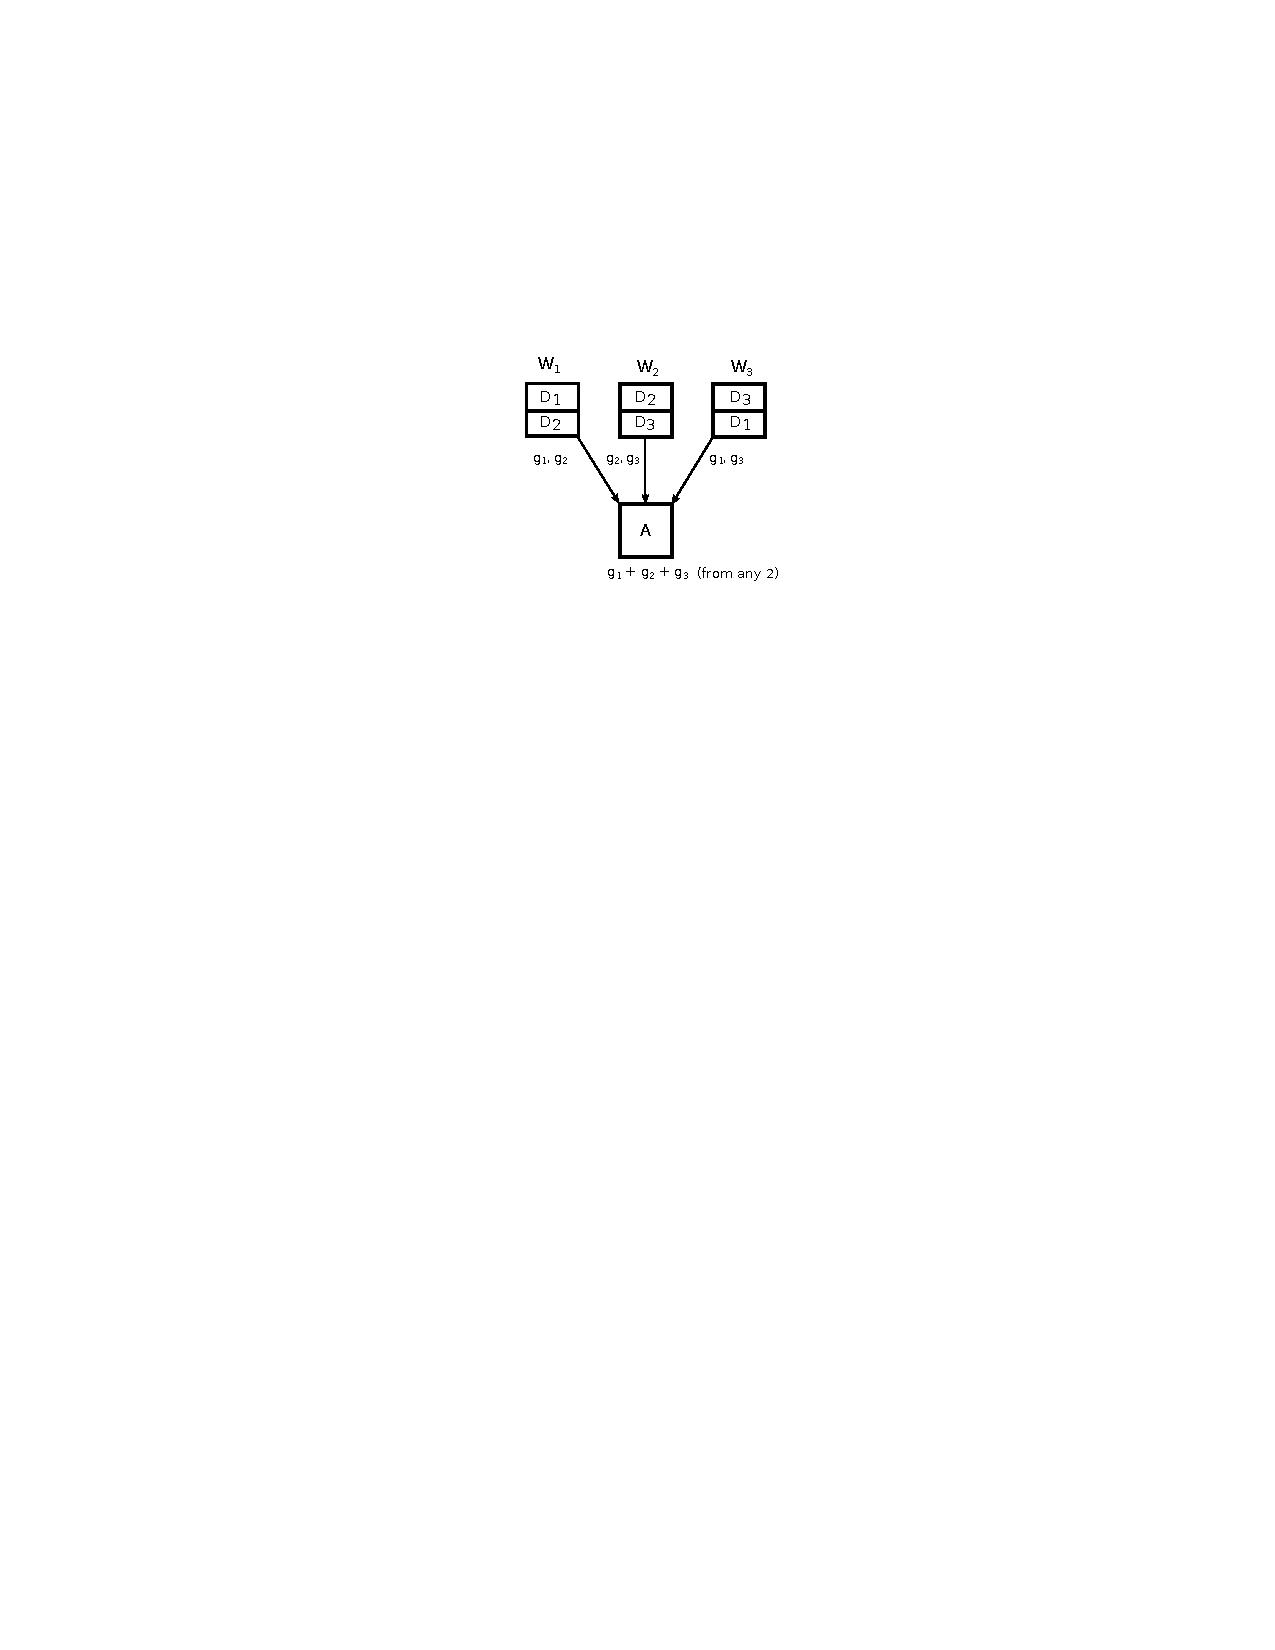
\includegraphics[height=.7\textheight]{res/replicate.pdf}
\end{figure}

Problem: high communication cost

\end{frame}

\begin{frame}{Distributed Learning}{Gradient Coding}

\begin{figure}
    \centering
    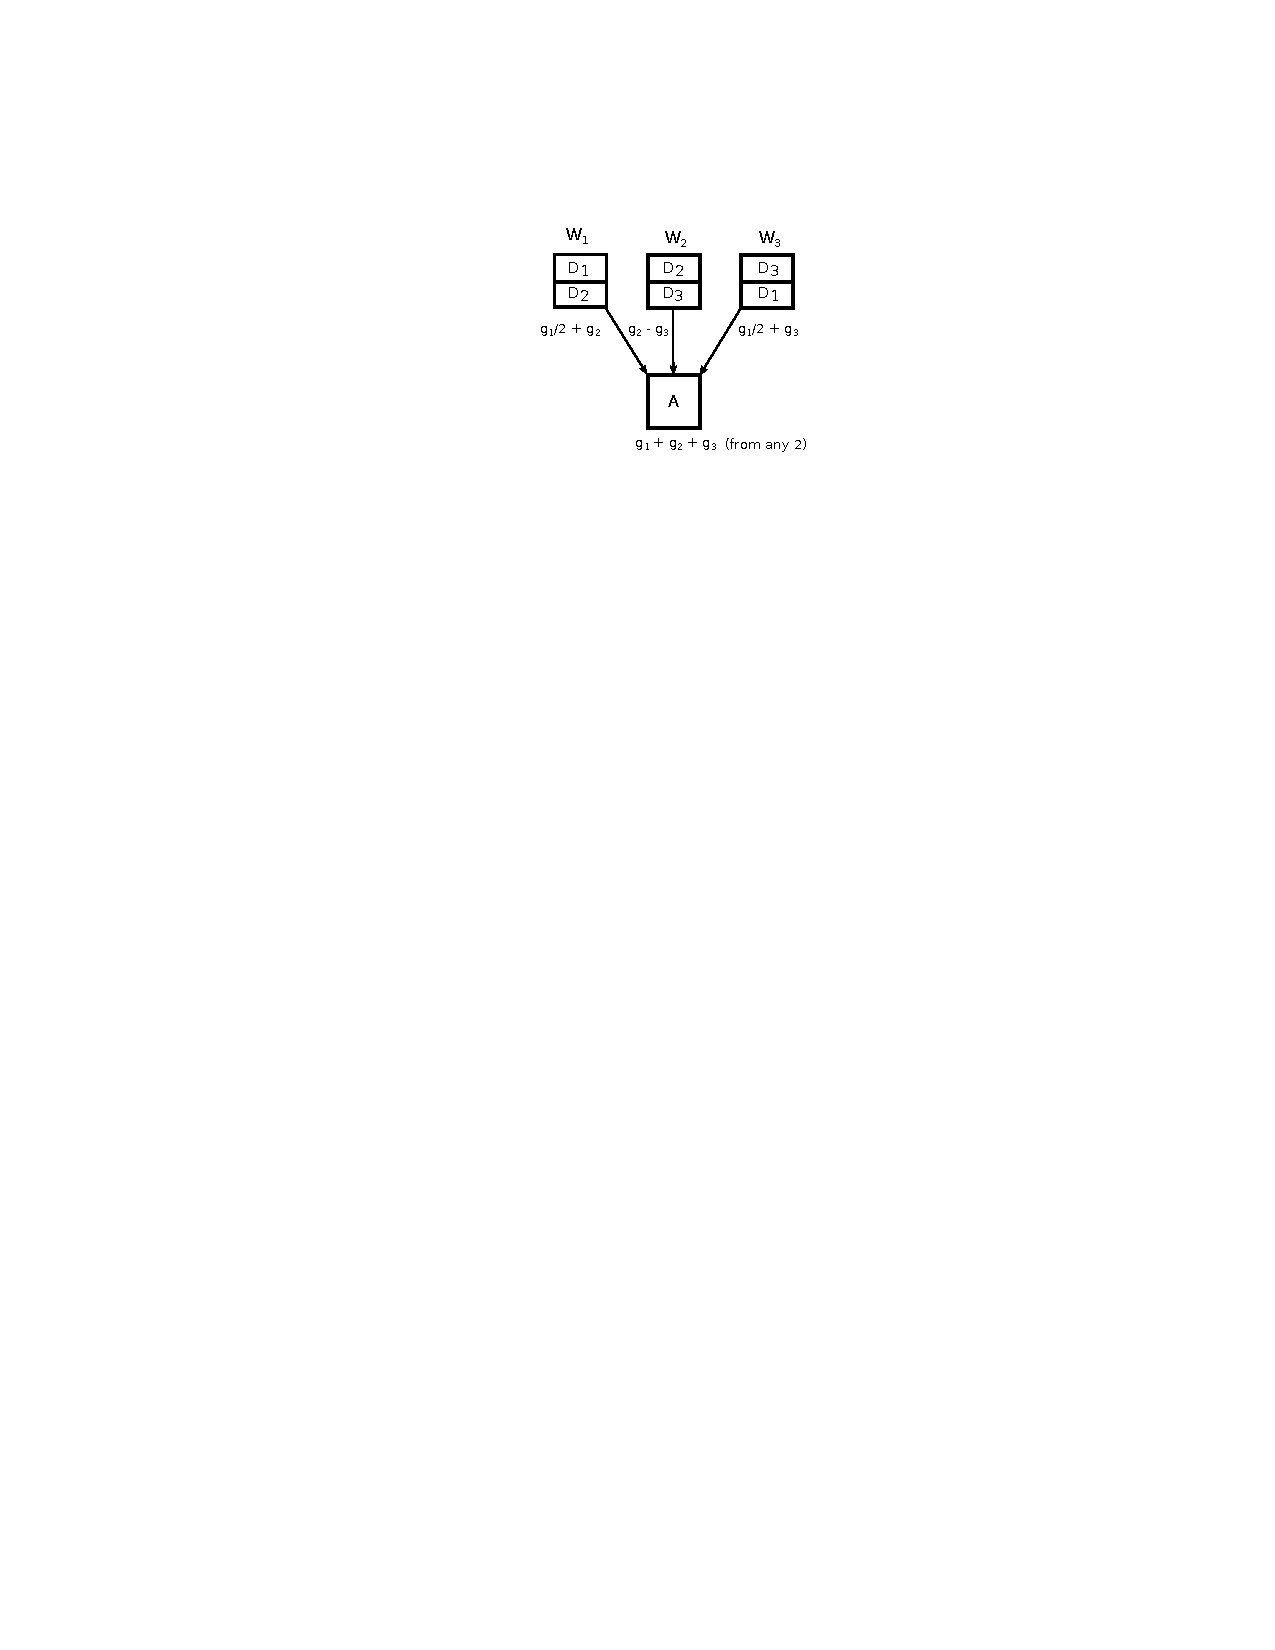
\includegraphics[height=.7\textheight]{res/gradient coding.pdf}
\end{figure}

\end{frame}

\section{Gradient Coding}

% \begin{frame}{Gradient Coding: Generalization}
%     \begin{columns}
%         \begin{column}{0.6\textwidth}
%             \begin{block}{Matrix Representation}
%                 \[B = \begin{bmatrix}
%                     \frac{1}{2} & 1 & 0 \\
%                     0 & 1 & -1 \\
%                     \frac{1}{2} & 0 & 1
%                 \end{bmatrix}, G = \begin{bmatrix}
%                     \boldsymbol{g_1}^T \\
%                     \boldsymbol{g_2}^T \\
%                     \boldsymbol{g_3}^T
%                 \end{bmatrix}\]
                
%                 \[BG = \begin{bmatrix}
%                     \frac{1}{2}\boldsymbol{g_1}^T + \boldsymbol{g_2}^T \\
%                     \boldsymbol{g_2}^T - \boldsymbol{g_3}^T \\
%                     \frac{1}{2}\boldsymbol{g_1}^T + \boldsymbol{g_3}^T
%                 \end{bmatrix}\]

%             \end{block}
%         \end{column}
%         \begin{column}{0.48\textwidth}
%             \begin{figure}
%                 \centering
%                 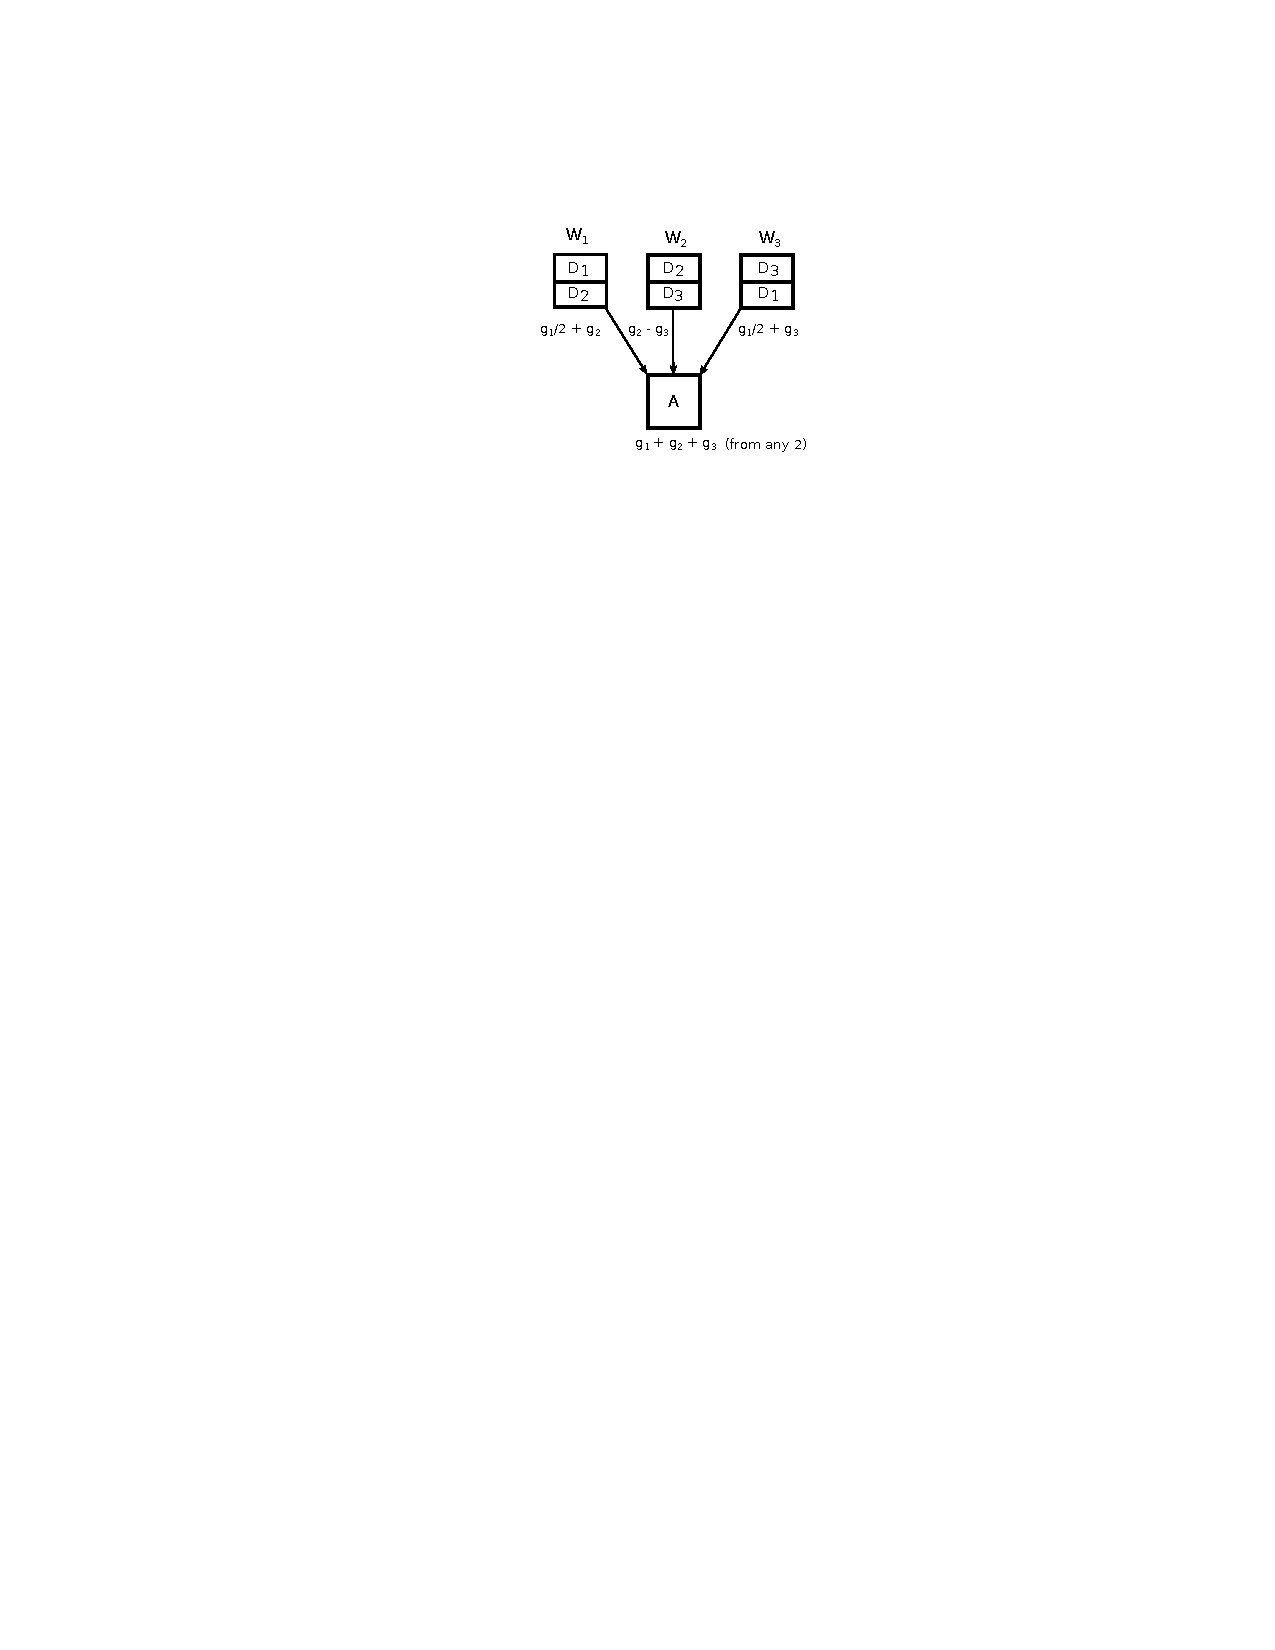
\includegraphics[height=.5\textheight]{res/gradient coding.pdf}
%             \end{figure}
%         \end{column}
%     \end{columns}
% \end{frame}

\begin{frame}{Definition of Notations}

\begin{definition}
    Let $f$ denotes the number of combinations of surviving workers/non-stragglers, $n$ denotes the number of workers, $k$ denotes the number of data partitions.
\end{definition}

\begin{definition}
    Let $A \in \mathbb{R}^{f \times n}$, the $i^{th}$ row of $A$ be $\boldsymbol{a}_i$. Each row of $A$ indicates a combination of surviving workers/non-stragglers.
\end{definition}

\begin{definition}
    Let $B \in \mathbb{R}^{n \times k}$, the $i^{th}$ row of $B$ be $\boldsymbol{b}_i$. $\boldsymbol{b}_i$ indicates the data partitions that the $i^{th}$ worker has access to.
\end{definition}

\end{frame}

\begin{frame}{Construction of $A$}

\begin{block}{Condition 1 (B-span)}
    Consider any scheme $(A, B)$ robust to any $s$ stragglers, given $n$ workers (with $s < n$). Then we require that for every subset $I \subseteq \{1, \dots, n\}, \lvert I \rvert = n - s$:
    \[\boldsymbol{1}_{1\times k} \in span\{\boldsymbol{b}_i \vert i \in I\}\]
    where $span\{·\}$ is the span of vectors.
\end{block}

\begin{lemma}
    Consider $B \in \mathbb{R}^{n\times k}$ satisfying Condition 1 for some $s < n$. Then there exists an $A \in \mathbb{R}^{\binom{n}{s}\times n}$ such that $AB = \boldsymbol{1}_{\binom{n}{s}\times n}$ and the scheme $(A, B)$ is robust to any s full stragglers.
\end{lemma}

\end{frame}

\begin{frame}{Lower Bound on $B$’s density}

\begin{theorem}
    Consider any scheme $(A, B)$ robust to any $s$ stragglers, given $n$ workers (with $s < n$) and $k$ partitions. Then, if all rows of $B$ have the same number of non-zeros, we must have: $\lVert b_i \rVert _0 >= \frac{k}{n}(s + 1)$ for any $i \in {1, \dots, n}$.
\end{theorem}

\begin{columns}

\begin{column}{.5\linewidth}
        
\begin{Example}
    \[A = \begin{bmatrix}
        0 & 1 & 2 \\
        1 & 0 & 1 \\
        2 & -1 & 0
    \end{bmatrix}\]
    
    \[B = \begin{bmatrix}
        1/2 & 1 & 0 \\
        0 & 1 & -1 \\
        1/2 & 0 & 1
    \end{bmatrix}\]
\end{Example}
    
\end{column}

\begin{column}{.5\linewidth}

\begin{figure}
    \centering
    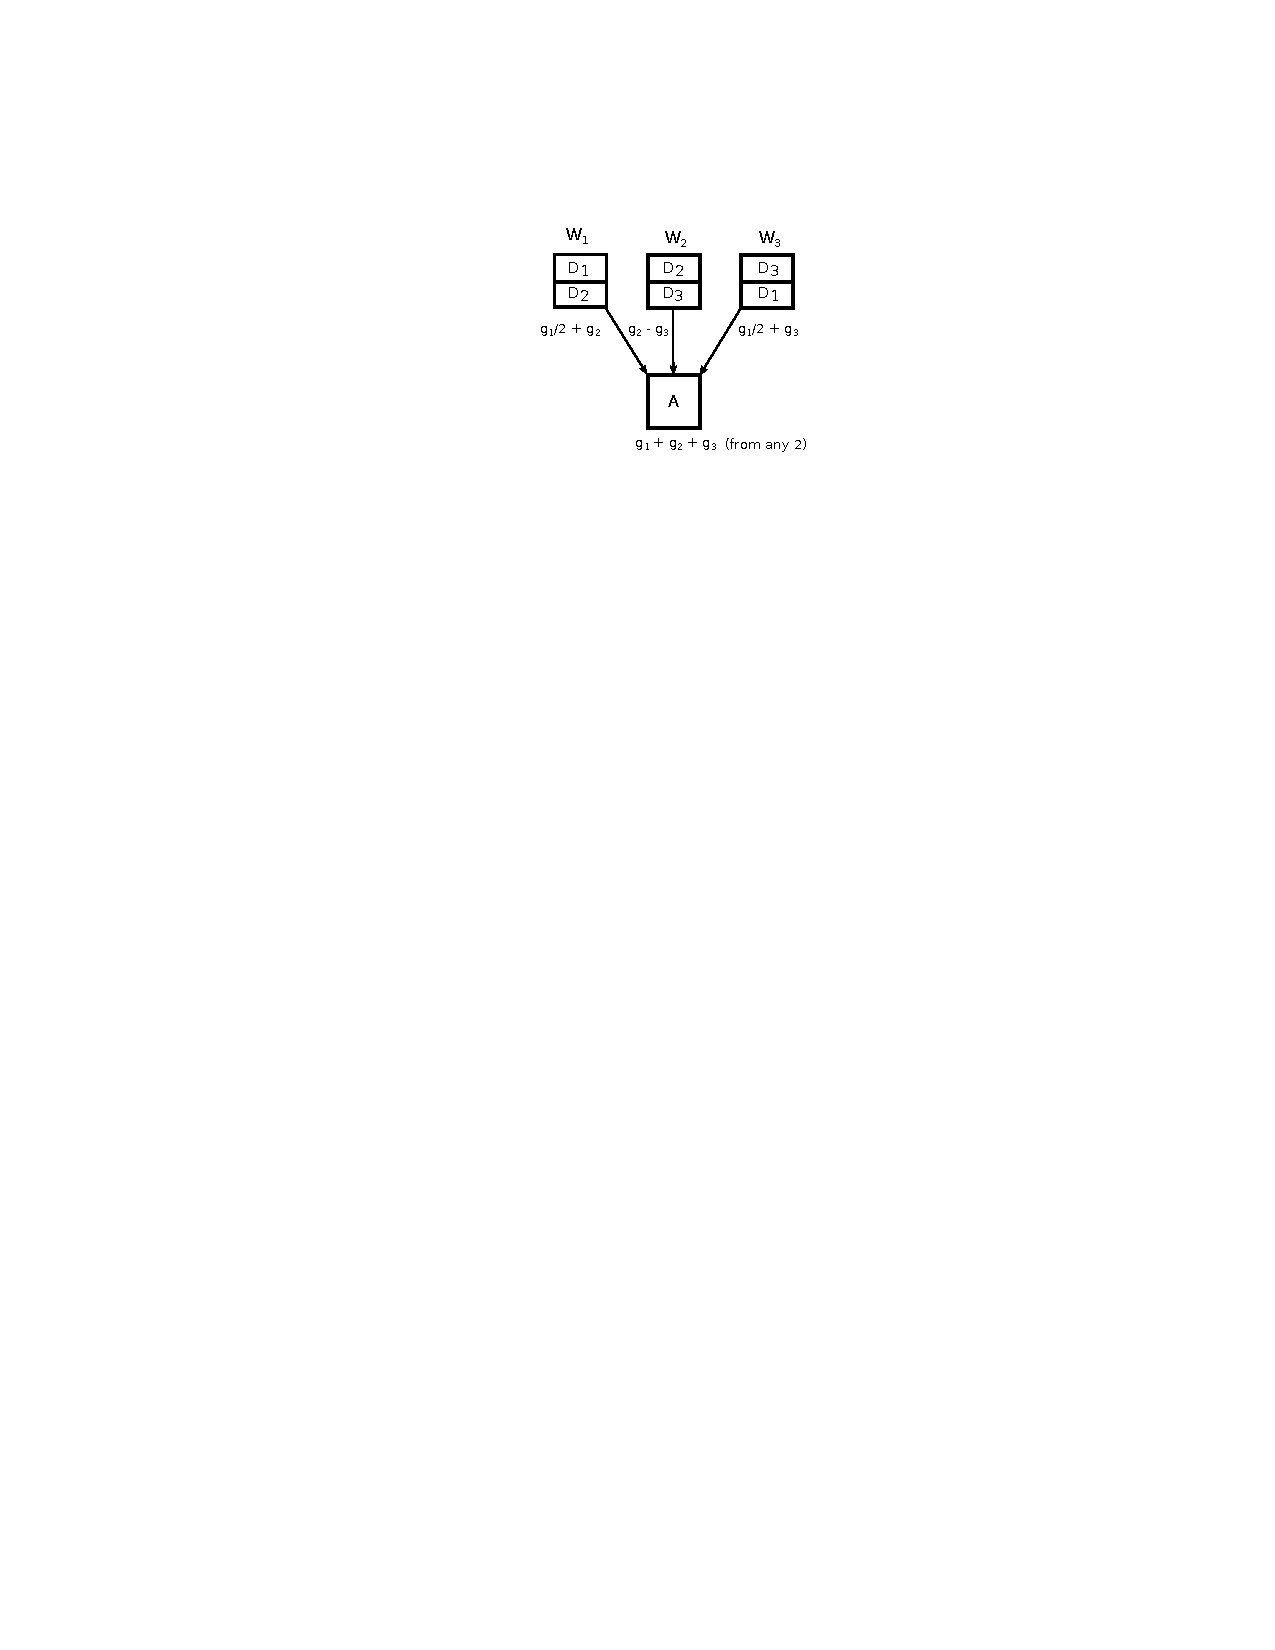
\includegraphics[width=\textwidth]{res/gradient coding.pdf}
\end{figure}

\end{column}

\end{columns}

\end{frame}

\begin{frame}{Fractional Repetition Scheme}
    \begin{block}{Construction of $B$}
        \[B = B_{frac} = \begin{bmatrix}
            \boldsymbol{1}_{(s+1)\times (s+1)} & \boldsymbol{0}_{(s+1)\times (s+1)} & \cdots & \boldsymbol{0}_{(s+1)\times (s+1)} \\
            \boldsymbol{0}_{(s+1)\times (s+1)} & \boldsymbol{1}_{(s+1)\times (s+1)} & \cdots & \boldsymbol{0}_{(s+1)\times (s+1)} \\
            \vdots & \vdots & \ddots & \vdots \\
            \boldsymbol{0}_{(s+1)\times (s+1)} & \boldsymbol{0}_{(s+1)\times (s+1)} & \cdots & \boldsymbol{1}_{(s+1)\times (s+1)}
        \end{bmatrix}_{n\times n}\]
    \end{block}

    \begin{theorem}
        Consider $B_{frac}$ constructed above, for a given number of workers $n$ and stragglers $s (< n)$. Then, $B_{frac}$ satisfies the B-Span condition (Condition 1). Consequently, the scheme $(A, B_{frac})$, with $A$ previously, is robust to any s stragglers.
    \end{theorem}
\end{frame}

\begin{frame}{Cyclic Repetition Scheme}
    \[B = B_{cyc} = \begin{bmatrix}
        \star & \star & \cdots & \star & \star & 0 & 0 & \cdots & 0 & 0 \\
        0 & \star & \cdots & \star & \star & \star & 0 & \cdots & 0 & 0 \\
        \vdots & \vdots & \vdots & \vdots & \vdots & \vdots & \ddots & \ddots & \vdots & \vdots \\
        0 & 0 & \cdots & 0 & 0 & \cdots & \star & \cdots & \star & \star \\
        \vdots & \vdots & \vdots & \vdots & \vdots & \vdots & \ddots & \ddots & \vdots & \vdots \\
        \star & \cdots & \star & \star & 0 & 0 & \cdots & 0 & 0 & \star
    \end{bmatrix}_{n\times n}\]
    ($s + 1$ non-zero elements in each row)

    \begin{block}{Construction}
        \begin{enumerate}
            \item Construct a random matrix $H \in \mathbb{R}^{s\times n}$ satisfying $H\boldsymbol{1} = \boldsymbol{0}$
            \item denote $S_i = \{i \mod n, \dots, (i + s) \mod n\}.$ for each $i$, let $b_i(i) = 1$, $b_i(S_i \backslash \{i\}) = -H_{S_i \backslash \{i\}}^{-1}H_i$
        \end{enumerate}
    \end{block}
\end{frame}

\begin{frame}{Cyclic Repetition SchemeL Construction Detail}
    \begin{block}{Construction Detail}
        \begin{enumerate}
            \item Construct a random matrix $H \in \mathbb{R}^{s\times n}$ satisfying $H\boldsymbol{1} = \boldsymbol{0}$
            
            Let $S$ be $H$'s null space. Then:
            \begin{itemize}
                \item Any $s$ columns of $H$ are linearly independent with probability $1$
                \item $dim(S) = n - s$ with probability $1$
                \item $\boldsymbol{1}\in S$, where $1$ is the all-ones vector
            \end{itemize}
            \item denote $S_i = \{i \mod n, \dots, (i + s) \mod n\}.$ for each $i$, let $b_i(i) = 1$, $b_i(S_i \backslash \{i\}) = -H_{S_i \backslash \{i\}}^{-1}H_i$

            Then:
            \begin{itemize}
                \item $b_i\in S$
                \item every element of $b_i(S_i \backslash \{i\})$ is non-zero with probability $1$
                \item for any subset $I\subseteq \{1, \dots, n\}$, $\lvert I\rvert = n - s$, the set of vectors $\{b_i \vert i\in I\}$ is linearly independent with probability $1$
            \end{itemize}
        \end{enumerate}
    \end{block}
\end{frame}

\section{Extends}

\begin{frame}
    \frametitle{Partial Stragglers}

    \begin{block}{Problem Setting}
        Each of the $s$ stragglers can finish work in $\alpha T$ time, while normal worker takes $T$ time.

        How to make use of stragglers?
    \end{block}

    \begin{solution}
        
        \begin{itemize}
            \item split the data $D$ into \textbf{naive} components and \textbf{coded} components
            \item all the workers process the \textbf{naive} components in normal way
            \item all the workers process the \textbf{coded} components using previous scheme
            \item size of \textbf{naive} components and \textbf{coded} components are $\frac{s + 1}{\alpha - 1} : 1$
        \end{itemize}
    \end{solution}

\end{frame}

\begin{frame}{DRACO}
    \begin{block}{Reference}
        L. Chen, H. Wang, Z. Charles, and D. Papailiopoulos, “\textbf{Draco: Byzantine-resilient distributed training via redundant gradients},” in International Conference on Machine Learning, PMLR, 2018, pp. 903–912.
    \end{block}

    \begin{block}{Main Idea}
        Replicate each data partition $2s+1$ times for $s$ stragglers.

        Decoding strategy:
        \begin{itemize}
            \item Fractional repetition scheme: finding the majority vote
            \item Cyclic repetition scheme: IDFT
        \end{itemize}
    \end{block}

\end{frame}

\begin{frame}{Trading Communication for Computation}
    \begin{block}{Reference}
        C. Hofmeister, L. Maßny, E. Yaakobi, and R. Bitar, “\textbf{Trading Communication for Computation in Byzantine-Resilient Gradient Coding},” arXiv preprint arXiv:2303.13231, 2023.
    \end{block}

    \begin{example}
        Setup: $g_1 = 1, g_2 = 2, g_3 = 3, g_4 = 4$, B is honest
        \begin{table}
            \begin{tabular}{llll}
            query                   & A   & B    & info                             \\
            $g_1 + g_2 + g_3 + g_4$ & $2$ & $10$ & $g_1 + g_2 + g_3 + g_4 = 2\ or\ 10$ \\
            $g_1 + g_2$             & $3$ & $3$  & $g_3 + g_4 = -1\ or\ 7$            \\
            $g_3$                   & $3$ & $3$  & $g_4 = -4\ or\ 4$                 
            \end{tabular}
        \end{table}
        $Oracle(g_4) = 4$: B is honest
    \end{example}
\end{frame}

\end{document}

